\documentclass[]{article}
% Imported Packages
%------------------------------------------------------------------------------
\usepackage{amssymb}
\usepackage{amstext}
\usepackage{amsthm}
\usepackage{amsmath}
\usepackage{enumerate}
\usepackage{fancyhdr}
\usepackage[margin=1in]{geometry}
\usepackage{graphicx}
\graphicspath{{../signatures/}}
\usepackage{multirow}
%\usepackage{extarrows}
%\usepackage{setspace}
%------------------------------------------------------------------------------

% Header and Footer
%------------------------------------------------------------------------------
\pagestyle{plain}  
\renewcommand\headrulewidth{0.4pt}                                      
\renewcommand\footrulewidth{0.4pt}                                    
%------------------------------------------------------------------------------
% Title Details
%------------------------------------------------------------------------------
\title{Deliverable \#1 Template : Software Requirement Specification (SRS)}
\author{SE 3A04: Software Design II -- Large System Design}
\date{10 March 2024}
                            
%------------------------------------------------------------------------------

% Document
%------------------------------------------------------------------------------
\begin{document}

\maketitle
\noindent{\bf Tutorial Number:} T01\\
{\bf Group Number:} G07 \\
{\bf Group Members:}
\begin{itemize}
	\item Awurama Nyarko
	\item Chelsea Maramot
	\item Harrison Chiu
	\item Khushi Bhojane
	\item Sumanya Gulati
\end{itemize}

\section*{IMPORTANT NOTES}
\begin{itemize}
	%	\item You do \underline{NOT} need to provide a text explanation of each diagram; the diagram should speak for itself
	\item Please document any non-standard notations that you may have used
	\begin{itemize}
		\item \emph{Rule of Thumb}: if you feel there is any doubt surrounding the meaning of your notations, document them
	\end{itemize}
	\item Some diagrams may be difficult to fit into one page
	\begin{itemize}
		\item Ensure that the text is readable when printed, or when viewed at 100\% on a regular laptop-sized screen.
		\item If you need to break a diagram onto multiple pages, please adopt a system of doing so and thoroughly explain how it can be reconnected from one page to the next; if you are unsure about this, please ask about it
	\end{itemize}
	\item Please submit the latest version of Deliverable 1 with Deliverable 2
	\begin{itemize}
		\item Indicate any changes you made.
	\end{itemize}
	\item If you do \underline{NOT} have a Division of Labour sheet, your deliverable will \underline{NOT} be marked
\end{itemize}

\newpage
\section{Introduction}
\label{sec:introduction}
% Begin Section

This section should provide an brief overview of the entire document.

\subsection{Purpose}
\label{sub:purpose}
% Begin SubSection
State the purpose and intended audience for the document.
% End SubSection

\subsection{System Description}
\label{sub:system_description}
% Begin SubSection
Give a brief description of the system. This could be a paragraph or two to give some context to this document.

% End SubSection

\subsection{Overview}
\label{sub:overview}
% Begin SubSection
Describe what the rest of the document contains and explain how the document is organised (e.g. "In Section 2 we discuss...in Section 3...").

% End SubSection

% End Section

\section{Analysis Class Diagram}
\label{sec:analysis_class_diagram}
% Begin Section
This section should provide an analysis class diagram for your application.
% End Section


\section{Architectural Design}
\label{sec:architectural_design}
% Begin Section
This section should provide an overview of the overall architectural design of your application. Your overall architecture should show the division of the system into subsystems with high cohesion and low coupling.

\subsection{System Architecture}
\label{sub:system_architecture}
% Begin SubSection
\begin{itemize}
	\item Identify and explain the overall architecture of your system
	\item Be sure to clearly state the name of the architecture you used (this is the name of the architectural pattern, not the name of your system)
	\item Provide the reasoning and justification of the choice of architecture
	\item Provide a structural architecture diagram showing the relationship among the subsystems (if appropriate)
	\item List any design alternatives you considered, but eliminated (and explain why you eliminated them)
\end{itemize}
% End SubSection

\subsection{Subsystems}
\label{sub:subsystems}
% Begin SubSection
 Provide a list of your subsystems, with a brief description of each. Be sure to document its purpose and relationship to other subsystems.

% End SubSection

% End Section
	
\section{Class Responsibility Collaboration (CRC) Cards}
\label{sec:class_responsibility_collaboration_crc_cards}
% Begin Section
This section should contain all of your CRC cards.

\begin{itemize}
	\item Provide a CRC Card for each identified class
	\item Please use the format outlined in tutorial, i.e., 
 
%CRC 1 - Authentication Management (Controller)
	\begin{table}[ht]
		\centering
		\begin{tabular}{|p{7cm}|p{7cm}|}
		\hline 
		 \multicolumn{2}{|l|}{\textbf{Class Name:} Account Management (Controller)} \\
		\hline
		\textbf{Responsibility:} & \textbf{Collaborators:} \\
		\hline
		Knows Account Success & knows Account Success\\
		Knows Account Error & Account Error \\
		Knows Create Account & Create Account\\
		Knows Login & Login\\
		Knows Change Status & Change Status\\
		Knows View Account & View Account\\
		Knows Account Database & Account Database\\
		Knows User Information &User Information\\
		Handles overall account-related functionalities
		\vspace{0.1in} & \\
		\hline
		\end{tabular}
	\end{table}

	\begin{table}[ht]
		\centering
		\begin{tabular}{|p{7cm}|p{7cm}|}
		\hline 
		 \multicolumn{2}{|l|}{\textbf{Class Name:} Account Success (Boundary)} \\
		\hline
		\textbf{Responsibility:} & \textbf{Collaborators:} \\
		\hline
		Knows Account Management & Account Management\\
		Handles unsuccessful events of saving and creating account
		\vspace{0.1in} & \\
		\hline
		\end{tabular}
	\end{table}

	\begin{table}[ht]
		\centering
		\begin{tabular}{|p{7cm}|p{7cm}|}
		\hline 
		 \multicolumn{2}{|l|}{\textbf{Class Name:} Account Error (Boundary)} \\
		\hline
		\textbf{Responsibility:} & \textbf{Collaborators:} \\
		\hline
		Knows Account Management & Account Management \\
		Knows Error Type &\\
		Knows Error Details &\\
		Handles account time-out event &\\
		Handles Creating Account error event &\\
		\vspace{0.1in} & \\
		\hline
		\end{tabular}
	\end{table}

	\begin{table}[ht]
		\centering
		\begin{tabular}{|p{7cm}|p{7cm}|}
		\hline 
		 \multicolumn{2}{|l|}{\textbf{Class Name:} Create Account (Boundary)} \\
		\hline
		\textbf{Responsibility:} & \textbf{Collaborators:} \\
		\hline
			Knows Account Management  & Account Management\\
			Knows Username &\\
			Knows Password &\\
			Knows Authorization and Permission Details &\\
			Handles validation of user-provided information for creating an account &\\
			Handles click-event of “Create Account” Button &\\
		\vspace{0.1in} & \\
		\hline
		\end{tabular}
	\end{table}

	\begin{table}[ht]
		\centering
		\begin{tabular}{|p{7cm}|p{7cm}|}
		\hline 
		 \multicolumn{2}{|l|}{\textbf{Class Name:} Edit Account (Boundary)} \\
		\hline
		\textbf{Responsibility:} & \textbf{Collaborators:} \\
		\hline
			Knows Account Management & Account Management\\
			Knows Username &\\
			Knows Password &\\
			Knows Authorization and Permission Details &\\
			Handles click-event of “Save” Button &\\
		\vspace{0.1in} & \\
		\hline
		\end{tabular}
	\end{table}

	\begin{table}[ht]
		\centering
		\begin{tabular}{|p{7cm}|p{7cm}|}
		\hline 
		 \multicolumn{2}{|l|}{\textbf{Class Name:} View Account(Boundary)} \\
		\hline
		\textbf{Responsibility:} & \textbf{Collaborators:} \\
		\hline
			Knows Account Management & Account Management \\
			Handles display of user account details to the user interface &\\
			Handles click-event of “View Account” button &\\
		\vspace{0.1in} & \\
		\hline
		\end{tabular}
	\end{table}

	\begin{table}[ht]
		\centering
		\begin{tabular}{|p{7cm}|p{7cm}|}
		\hline 
		 \multicolumn{2}{|l|}{\textbf{Class Name:} Login(Boundary)} \\
		\hline
		\textbf{Responsibility:} & \textbf{Collaborators:} \\
		\hline
			Knows Account Management & Account Management\\
			Knows Authentication and Authorization details &\\
			Handles validation of user login credentials &\\
			Handles click event of “login” button &\\
		\vspace{0.1in} & \\
		\hline
		\end{tabular}
	\end{table}

	\begin{table}[ht]
		\centering
		\begin{tabular}{|p{7cm}|p{7cm}|}
		\hline 
		 \multicolumn{2}{|l|}{\textbf{Class Name:} Current Status (Boundary)} \\
		\hline
		\textbf{Responsibility:} & \textbf{Collaborators:} \\
		\hline
			Knows Account Management & Account Management \\
			Knows User Availability Status (e.g., online, away, do not disturb, custom, in a meeting) &\\
			Handles updates of current User Availability Status &\\
		\vspace{0.1in} & \\
		\hline
		\end{tabular}
	\end{table}

	\begin{table}[ht]
		\centering
		\begin{tabular}{|p{7cm}|p{7cm}|}
		\hline 
		 \multicolumn{2}{|l|}{\textbf{Class Name:} Account Database (Entity)} \\
		\hline
		\textbf{Responsibility:} & \textbf{Collaborators:} \\
		\hline
			Knows Account Management & Account Management \\
			Knows User Information & User Information \\
			Knows Account Permissions &\\
			Knows Account Status &\\
			Handles storage of user account data &\\
		\vspace{0.1in} & \\
		\hline
		\end{tabular}
	\end{table}

	\begin{table}[ht]
		\centering
		\begin{tabular}{|p{7cm}|p{7cm}|}
		\hline 
		 \multicolumn{2}{|l|}{\textbf{Class Name:} User Information (Entity)} \\
		\hline
		\textbf{Responsibility:} & \textbf{Collaborators:} \\
		\hline

			Knows Account Management & Account Management \\
			Knows Account Database & Account Database \\
			Knows Username &\\
			Knows Password &\\
			Knows Gender &\\
			Knows Team Manager &\\
			Knows Company Name &\\
			Knows Date-of-Birth &\\
			Handles storage and management of user specific details &\\
		\vspace{0.1in} & \\
		\hline
		\end{tabular}
	\end{table}

	\begin{table}[ht]
		\centering
		\begin{tabular}{|p{7cm}|p{7cm}|}
		\hline 
		 \multicolumn{2}{|l|}{\textbf{Class Name:} File Management (Controller)} \\
		\hline
		\textbf{Responsibility:} & \textbf{Collaborators:} \\
		\hline
			Knows File Name & Chat Management Controller\\
			Knows File Size & File Database\\
			Knows File Type &\\
			Knows File Permissions &\\
			Handles coordination of sending, receiving, and storage of files &\\
			Handles the enforcement of file access permission &\\
		\vspace{0.1in} & \\
		\hline
		\end{tabular}
	\end{table}


	\begin{table}[ht]
		\centering
		\begin{tabular}{|p{7cm}|p{7cm}|}
		\hline 
		 \multicolumn{2}{|l|}{\textbf{Class Name:} File Database (Entity)} \\
		\hline
		\textbf{Responsibility:} & \textbf{Collaborators:} \\
		\hline
			Knows File Management & File Management \\
			Knows File Name &\\
			Knows File Size &\\
			Knows File Type &\\
			Knows File Permissions &\\
			Knows File Owner &\\
			Handles the storage of file data &\\
		\vspace{0.1in} & \\
		\hline
		\end{tabular}
	\end{table}


	\begin{table}[ht]
		\centering
		\begin{tabular}{|p{7cm}|p{7cm}|}
		\hline 
		 \multicolumn{2}{|l|}{\textbf{Class Name:} File Search (Boundary)} \\
		\hline
		\textbf{Responsibility:} & \textbf{Collaborators:} \\
		\hline
			Knows File Management & File Management\\
			Knows File Search Criteria (e.g., File Name, File Type, File Owner) &\\
			Handles file search functionality &\\
			Handles utilization of search criteria to locate and retrieve files matching specified conditions &\\
			Handles click-event of “Search” button &\\
		\vspace{0.1in} & \\
		\hline
		\end{tabular}
	\end{table}

	\begin{table}[ht]
		\centering
		\begin{tabular}{|p{7cm}|p{7cm}|}
		\hline 
		 \multicolumn{2}{|l|}{\textbf{Class Name:} File Retrieval (Boundary)} \\
		\hline
		\textbf{Responsibility:} & \textbf{Collaborators:} \\
		\hline
			Knows File Management & File Management \\
			Knows File ID & File Search \\
			Knows File Name &\\
			Knows File Type &\\
			Knows File Owner &\\
			Handles retrieval of files from storage based on specified file search criteria &\\
		\vspace{0.1in} & \\
		\hline
		\end{tabular}
	\end{table}

	\begin{table}[ht]
		\centering
		\begin{tabular}{|p{7cm}|p{7cm}|}
		\hline 
		 \multicolumn{2}{|l|}{\textbf{Class Name:} File Error (Boundary)} \\
		\hline
		\textbf{Responsibility:} & \textbf{Collaborators:} \\
		\hline
			Knows File Management & File Management \\
			Knows Error Type &\\
			Knows Error Details &\\
			Handles errors related to file operations (e.g., Invalid File Type Error, File Size Too Big) &\\
			Handles communication of error information to the user &\\
		\vspace{0.1in} & \\
		\hline
		\end{tabular}
	\end{table}

	\begin{table}[ht]
		\centering
		\begin{tabular}{|p{7cm}|p{7cm}|}
		\hline 
		\multicolumn{2}{|l|}{\textbf{Class Name:} Chat History Database (Entity)} \\
		\hline
		\textbf{Responsibility:} & \textbf{Collaborators:} \\
		\hline
  			Knows Chat Management Controller & Chat Management Controller \\
     			Knows User Info & User Info \\
			Knows Send Message & Send Message \\
			Knows Send Files & Send Files \\
			Knows Delete/Edit Message & Delete/Edit Message\\
			Knows Disappearing Message & Disappearing Message \\
			Handles Load Previous Message events & \\
		\vspace{1in} & \\
		\hline
		\end{tabular}
	\end{table}

  	\begin{table}[ht]
		\centering
		\begin{tabular}{|p{7cm}|p{7cm}|}
		\hline 
		\multicolumn{2}{|l|}{\textbf{Class Name:} Create Group (Boundary)} \\
		\hline
		\textbf{Responsibility:} & \textbf{Collaborators:} \\
		\hline
  			Knows Chat Management Controller & Chat Management Controller \\
			Knows Edit Group Members & Edit Group Members \\
			Knows Edit Group Details & Edit Group Details \\
			Knows User Info & User Info \\
			Handles new group creation events &\\
		\vspace{1in} & \\
		\hline
		\end{tabular}
	\end{table}

   	\begin{table}[ht]
		\centering
		\begin{tabular}{|p{7cm}|p{7cm}|}
		\hline 
		\multicolumn{2}{|l|}{\textbf{Class Name:} Edit Group Members (Boundary)} \\
		\hline
		\textbf{Responsibility:} & \textbf{Collaborators:} \\
		\hline
  			Knows Chat Management Controller & Chat Management Controller \\
			Knows User Info & User Info \\
			Handles events pertaining to the addition/removal of members from a group chat &\\
		\vspace{1in} & \\
		\hline
		\end{tabular}
	\end{table}

   	\begin{table}[ht]
		\centering
		\begin{tabular}{|p{7cm}|p{7cm}|}
		\hline 
		\multicolumn{2}{|l|}{\textbf{Class Name:} Edit Group Details (Boundary)} \\
		\hline
		\textbf{Responsibility:} & \textbf{Collaborators:} \\
		\hline
  			Knows Chat Management Controller & Chat Management Controller \\
			Knows Create Group & Create Group \\
			Handles events related to editing group chat details including name, description and picture. &\\
		\vspace{1in} & \\
		\hline
		\end{tabular}
	\end{table}

    	\begin{table}[ht]
		\centering
		\begin{tabular}{|p{7cm}|p{7cm}|}
		\hline 
		\multicolumn{2}{|l|}{\textbf{Class Name:} Message Error (Boundary)} \\
		\hline
		\textbf{Responsibility:} & \textbf{Collaborators:} \\
		\hline
  			Knows Chat Management Controller & Chat Management Controller \\
			Knows Send Message & Send Message \\
			Knows Delete/Edit Message & Delete/Edit Message \\
			Knows Disappearing Message & Disappearing Message \\
			Knows Delivered Status Message & Delivered Status Message \\
   			Handles unsuccessful events of sending a message. &\\
			Handles unsuccessful events of deleting or editing a message past the set time limit. &\\
			Handles unsuccessful events of viewing a disappearing message after it has been read. &\\
		\vspace{1in} & \\
		\hline
		\end{tabular}
	\end{table}

    	\begin{table}[ht]
		\centering
		\begin{tabular}{|p{7cm}|p{7cm}|}
		\hline 
		\multicolumn{2}{|l|}{\textbf{Class Name:} Chat Management Controller} \\
		\hline
		\textbf{Responsibility:} & \textbf{Collaborators:} \\
		\hline
  			Knows File Management Controller & File Management Controller \\
			Knows Send Message & Send Message \\
			Knows Send Files & Send Files \\
			Knows Delete/Edit Message & Delete/Edit Message \\
			Knows Disappearing Message & Disappearing Message \\
			Knows Load Previous Message & Load Previous Message \\
			Knows Delivered Status Message & Delivered Status Message \\
			Knows Chat History Database & Chat History Database \\
			Knows Create Group & Create Group \\
			Knows Edit Group Members & Edit Group Members \\
			Knows Edit Group Details & Edit Group Details \\
			Knows Message Error & Message Error \\
		\vspace{1in} & \\
		\hline
		\end{tabular}
	\end{table}

    	\begin{table}[ht]
		\centering
		\begin{tabular}{|p{7cm}|p{7cm}|}
		\hline 
		\multicolumn{2}{|l|}{\textbf{Class Name:} File Permissions (Boundary)} \\
		\hline
		\textbf{Responsibility:} & \textbf{Collaborators:} \\
		\hline
  			Knows File Management Controller & File Management Controller \\
			Knows File Name & File Name \\
			Knows File Owner & File Owner \\
			Knows File Database & File Database \\
			Knows File Access & File Access \\
			Knows File Error Handling & File Error Handling \\
			Handles setting permission for file access events. &\\
		\vspace{1in} & \\
		\hline
		\end{tabular}
	\end{table}

     	\begin{table}[ht]
		\centering
		\begin{tabular}{|p{7cm}|p{7cm}|}
		\hline 
		\multicolumn{2}{|l|}{\textbf{Class Name: Authentication Management (Controller)
		}} \\
		\hline
		\textbf{Responsibility:} & \textbf{Collaborators:} \\
		\hline
            Knows Account Management & Account Management\\
            
            Knows User Information & User Information\\
            Knows Username & Encryption\\
            Knows Password\
            
            \vspace{0.1in}
            \textbf{Handles token generation which will be used by the user to access their account.}

		\vspace{1in} & \\
		\hline
  
		\end{tabular}
	\end{table}
 

 %CRC 2 - Token Generation (Entity)
	\begin{table}[ht]
		\centering
		\begin{tabular}{|p{7cm}|p{7cm}|}
		\hline 
		 \multicolumn{2}{|l|}{\textbf{Class Name: Token Generation (Entity)
}} \\
		\hline
		\textbf{Responsibility:} & \textbf{Collaborators:} \\
		\hline
            Knows Account Management & Authentication Management\\
            
            Knows User Information & Account Management\\
            & Encryption\\
            
            \vspace{0.1in}
            \textbf{Handles the generation of a token which will be used by the user to access their account.}

		\vspace{1in} & \\
		\hline
  
		\end{tabular}
	\end{table}

 %CRC 3 - Encryption (Boundary)
	\begin{table}[ht]
		\centering
		\begin{tabular}{|p{7cm}|p{7cm}|}
		\hline 
		 \multicolumn{2}{|l|}{\textbf{Class Name: Encryption (Boundary)
}} \\
		\hline
		\textbf{Responsibility:} & \textbf{Collaborators:} \\
		\hline
            Knows Chat Management & Authentication Management\\
            Knows User Information & Account Management\\
            Knows Authentication Management & User Information\\
            Knows Account Management
            
            \vspace{0.1in}
            \textbf{Handles the overall security and encryption of user data and messages being sent as well as company data.}

		\vspace{1in} & \\
		\hline
  
		\end{tabular}
	\end{table}

 %CRC 4 - Send Message (Boundary)
	\begin{table}[ht]
		\centering
		\begin{tabular}{|p{7cm}|p{7cm}|}
		\hline 
		 \multicolumn{2}{|l|}{\textbf{Class Name: Send Message (Boundary)
}} \\
		\hline
		\textbf{Responsibility:} & \textbf{Collaborators:} \\
		\hline
            Knows Message Contents and Type & Chat Management\\
            Knows Message Permissions & File Management\\
            & Encryption\\
            
            \vspace{0.1in}
            \textbf{Handles the sending of messages between accounts.}

		\vspace{1in} & \\
		\hline
  
		\end{tabular}
	\end{table}

 
 %CRC 5 - Send Files (Boundary)
	\begin{table}[ht]
		\centering
		\begin{tabular}{|p{7cm}|p{7cm}|}
		\hline 
		 \multicolumn{2}{|l|}{\textbf{Class Name: Send Files (Boundary)
}} \\
		\hline
		\textbf{Responsibility:} & \textbf{Collaborators:} \\
		\hline
            Knows Name & File Management\\
            Knows File Size & Chat Management\\
            Knows File Type & Encryption\\
            Knows File Permissions\\
            
            \vspace{0.1in}
            \textbf{Handles the sending of files between accounts.}

		\vspace{1in} & \\
		\hline
  
		\end{tabular}
	\end{table}

 %CRC 6 - Delete/Edit Messages (Boundary)
	\begin{table}[ht]
		\centering
		\begin{tabular}{|p{7cm}|p{7cm}|}
		\hline 
		 \multicolumn{2}{|l|}{\textbf{Class Name: Delete/Edit Messages (Boundary)
}} \\
		\hline
		\textbf{Responsibility:} & \textbf{Collaborators:} \\
		\hline
            Knows Message Contents and Type & Chat Management\\
            Knows Message Permissions & File Management\\
            & Encryption\\
            
            \vspace{0.1in}
            \textbf{Handles the deletion and editing of messages between accounts.}

		\vspace{1in} & \\
		\hline
  
		\end{tabular}
	\end{table}

 %CRC 7 - Disappearing Messages - Set Time (Boundary)
	\begin{table}[ht]
		\centering
		\begin{tabular}{|p{7cm}|p{7cm}|}
		\hline 
		 \multicolumn{2}{|l|}{\textbf{Class Name: Disappearing Messages - Set Time (Boundary)
}} \\
		\hline
		\textbf{Responsibility:} & \textbf{Collaborators:} \\
		\hline
            Knows Message Contents and Type & Chat Management\\
            Knows Message Permissions & File Management\\
            & Encryption\\
            
            \vspace{0.1in}
            \textbf{Handles the disappearing of messages after a set time.}

		\vspace{1in} & \\
		\hline
  
		\end{tabular}
	\end{table}


 %CRC 8 - Load Previous Message (Boundary)
	\begin{table}[ht]
		\centering
		\begin{tabular}{|p{7cm}|p{7cm}|}
		\hline 
		 \multicolumn{2}{|l|}{\textbf{Class Name: Load Previous Message (Boundary)
}} \\
		\hline
		\textbf{Responsibility:} & \textbf{Collaborators:} \\
		\hline
            Knows Message Contents and Type & Chat Management\\
            Knows Message Permissions & File Management\\
            & Encryption\\
            
            \vspace{0.1in}
            \textbf{Handles the storage and loading of previous messages.}

		\vspace{1in} & \\
		\hline
  
		\end{tabular}
	\end{table}


 %CRC 9 - Delivered Status Message (Boundary)
	\begin{table}[ht]
		\centering
		\begin{tabular}{|p{7cm}|p{7cm}|}
		\hline 
		 \multicolumn{2}{|l|}{\textbf{Class Name: Delivered Status Message (Boundary)
}} \\
		\hline
		\textbf{Responsibility:} & \textbf{Collaborators:} \\
		\hline
            Knows Message Contents and Type & Chat Management\\
            Knows Message Permissions & Encryption\\
            \vspace{0.1in}
            \textbf{Handles the storage and loading of previous messages.}

		\vspace{1in} & \\
		\hline
  
		\end{tabular}
	\end{table}
\end{itemize}



% End Section
\clearpage

\clearpage

\appendix
\section{Division of Labour}
\label{sec:division_of_labour}
% Begin Section
Include a Division of Labour sheet which indicates the contributions of each team member. This sheet must be signed by all team members.
% End Section
\subsection{Awurama Nyarko}
\label{subsec:awurama_nyarko}
\begin{itemize}
	\item 1.1 Purpose
	\item 1.2 System Description
	\item 1.3 Overview
	\item 3.1 System Architecture: explained used of MVC and Repository
\end{itemize}
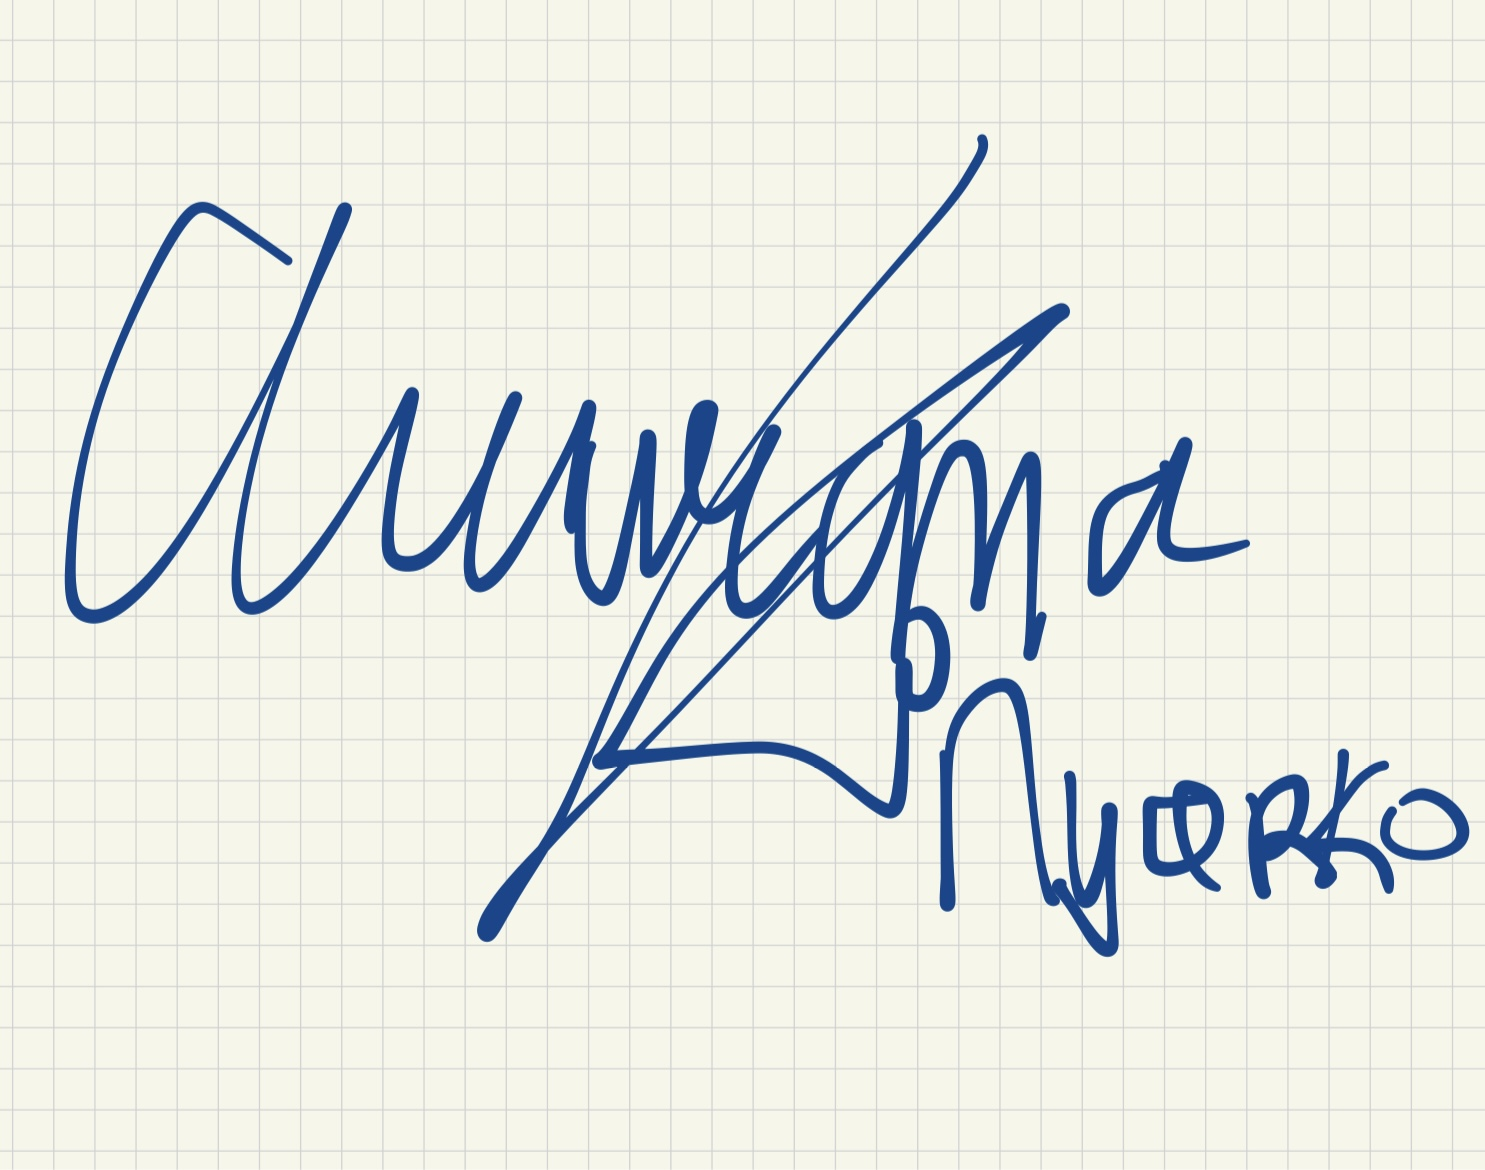
\includegraphics[width=0.5\textwidth]{awurama.jpg}

\subsection{Chelsea Maramot}
\label{subsec:chelsea_maramot}
\begin{itemize}
	\item Figure 1. Part of Analysis Class Diagram
	\item Class Responsibility Collaboration (CRC) cards
 		\begin{itemize}
   			\item File Management: File Error Handling
      			\item File Management: File Access
	 		\item File Management: File Search and Retrieval
    			\item Account Management: Account Management
       			\item Account Management: Account Database
	  		\item Account Management: User Information
     			\item Account Management: Log-in/Sign-in
			\item Account Management: Change Status
   			\item Account Management: View Account
      		\end{itemize}
\end{itemize}
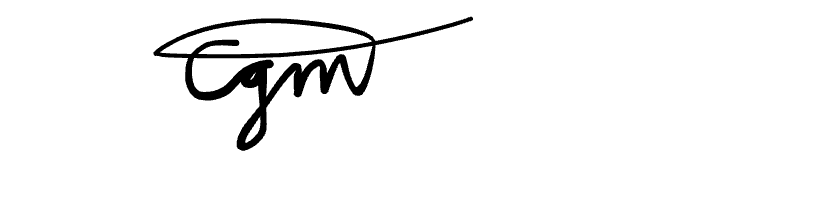
\includegraphics[width=0.5\textwidth]{chelsea.png}

\subsection{Harrison Chiu}
\label{subsec:harrison_chiu}
\begin{itemize}
	\item 3.1 System Architetcure: explained elimiation of other architecture designs
	\item Figure 2. System Architecture
 	\item 3.2 Subsystems
\end{itemize}

\includegraphics[width=0.5\textwidth]{harrison.png}

\subsection{Khushi Bhojane}
\label{subsec:khushi_bhojane}
\begin{itemize}
	\item Figure 1. Part of Analysis Class Diagram
	\item Class Responsibility Collaboration (CRC) cards
 		\begin{itemize}
   			\item Authentication Management: Encryption
      			\item Authentication Management: Token Generation
	 		\item Authentication Management: Authentication Management
    			\item Chat Management: Send Message
       			\item Chat Management: Send Files
	  		\item Chat Management: Edit/Delete Message
     			\item Chat Management: Disappearing/Vanishing Messages
			\item Chat Management: Load Previous Messages
   			\item Chat Management: 'Delivered' Status Message
      		\end{itemize}
\end{itemize}
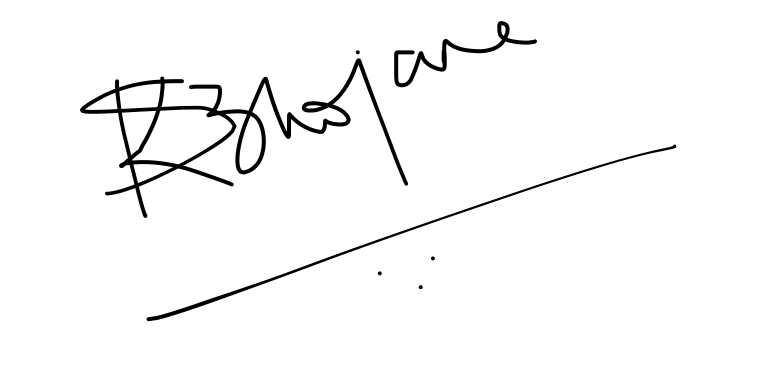
\includegraphics[width=0.5\textwidth]{khushi_signature.png}

\subsection{Sumanya Gulati}
\label{subsec:sumanya_gulati}
\begin{itemize}
	\item Figure 1. Part of Analysis Class Diagram
	\item Class Responsibility Collaboration (CRC) cards
 		\begin{itemize}
   			\item Chat Management: Chat History Database
      			\item Chat Management: Create Group
	 		\item Chat Management: Edit Group Members
    			\item Chat Management: Edit Group Details
       			\item Chat Management: Message Error
	  		\item Chat Management: Chat Management
     			\item File Management: File Management
			\item File Management: File Permissions
      		\end{itemize}
\end{itemize}

\includegraphics[width=0.5\textwidth]{signature.jpeg}

\end{document}
%------------------------------------------------------------------------------
